\documentclass[conference]{IEEEtran}
\IEEEoverridecommandlockouts
% The preceding line is only needed to identify funding in the first footnote. If that is unneeded, please comment it out.
\usepackage{cite}
\usepackage{amsmath,amssymb,amsfonts}
\usepackage{algorithmic}
\usepackage{graphicx}
\usepackage{url}
\usepackage[utf8]{inputenc}
\usepackage{textcomp}


\usepackage[english,ngerman,brazilian]{babel}
\def\BibTeX{{\rm B\kern-.05em{\sc i\kern-.025em b}\kern-.08em
    T\kern-.1667em\lower.7ex\hbox{E}\kern-.125emX}}
\begin{document}

\title{Projeto Demonstrativo 3 - Múltiplas Vistas}

\author{\IEEEauthorblockN{Frederico Guth (18/0081641)}
\IEEEauthorblockA{\textit{Tópicos em Sistemas de Computação, ,} \\
\textit{Turma TC - Visão Computacional (PPGI)}\\
\textit{Universidade de Brasília}\\
Brasília, Brasil\\
fredguth@fredguth.com}
}

\maketitle

\begin{abstract}
Uma câmera faz um mapeamento geométrico do mundo para uma imagem e é possível, fazer o caminho inverso, mapeando a posição de objetos no mundo a partir da sua imagem. Para isso, entretanto, é preciso conhecer os parâmetros intrínsecos e extrínsecos da câmera, o que chamamos de calibração. Neste projeto mostramos como calibrar a câmera e obter informações do mundo 3D a partir de imagens.
\end{abstract}

\begin{IEEEkeywords}
câmeras, calibração, parâmetros intrísecos, parâmetros extrínsecos, projeção reversa
\end{IEEEkeywords}

\section{Introdução}
A extração de informações 3D de uma cena a partir de imagens 2D pode ser obtida por uma triangulação (Apêndice A.5.3), em que a posição 3D (profundidade) relativa a um par de pontos correspondentes1 entre duas imagens é calculada. O mapa de profundidade, também conhecido como imagem de profundidade, armazena os valores de profundidade estimados para cada ponto de uma imagem 2D, representando a estrutura 3D da cena. A Figura 13 (c) mostra o mapa de profundidade computado por uma triangulação dos pontos correspondentes e não ocluídos das imagens ilustradas na Figura 13 (a) e (b). As áreas mais claras do mapa de profundidade representam as superfícies dos objetos mais próximas do plano da imagem, enquanto as áreas escuras, as superfícies mais distantes.
A profundidade calculada pela triangulação requer que a correspondência de pontos entre um par de imagens seja estimada. Tradicionalmente, a busca por pontos correspondentes é realizada levando em consideração a restrição epipolar (Apêndice A.5), a qual estabelece que, dado um ponto x da primeira vista, a busca por um ponto x′ correspondente na segunda vista não precisa cobrir toda a imagem e restringe-se apenas a uma linha epipolar. A busca pode ser aprimorada empregando imagens retificadas. A retificação de um par de imagens transforma cada plano das imagens de forma que as linhas epipolares se tornem colineares e paralelas horizontalmente [6], permitindo que a busca seja realizada ao longo das linhas horizontais das imagens retificadas, aumentando o desempenho computacional [24].
Na busca por pontos correspondentes, empregando um par de imagens retificadas, a medida de disparidade d, que é a diferença entre os pontos correspondentes das imagens da esquerda e direita, pode ser usada para obter o valor de profundidade z, pela relação definida em [29] como
d = bf 1 (66) z
em que b é a distância entre os centros de projeção das câmeras (baseline) e f é a distância focal. Um algoritmo básico para estimação de um mapa de profundidade entre um par de imagens retificadas é apresentado em [25, 29] e descrito a seguir. Considerando o pixel p1 da primeira imagem I1 (imagem de referência), a busca pelo ponto correspondente p2 na segunda imagem
1Dados dois pontos x e x′, eles são ditos correspondentes se existir um ponto X no espaço 3D, o qual é projetado para o ponto x, em uma primeira vista, e x′ em uma segunda vista [13].
  26
   (a) (b) (c)
Figura 13: Mapa de profundidade (imagem (c)) gerado por uma triangulação dos pontos corres- pondentes das imagens (a) e (b). Fonte: [25].
I2 é realizada ao longo da linha horizontal, em que a similaridade entre p1 e p2 é medida pela comparação entre blocos W que cercam os pixels, como ilustra a Figura 14. A similaridade (correlação) dos blocos pode ser medida pela soma das diferenças absolutas e a disparidade d de um pixel na posição (x, y) na imagem I1 pode ser calculada como
􏰆􏰁 ̃􏰁
d(x,y)= arg min 􏰁􏰁I1(x+i,y+j)−I2(x+i−d,y+j)􏰁􏰁 (67)
 ̃
0≤d≤dmax (i,j)∈W
em que dmax representa a disparidade máxima, limitando a busca, d ̃ é a disparidade candidata para um determinado par de blocos, i e j definem as coordenadas dos pixels pertencentes aos blocos e d(x,y) é a disparidade computada para o pixel na posição (x,y) da imagem I1, com relação à menor diferença de similaridade entre os blocos comparados. A partir da disparidade d computada, a profundidade pode ser obtida pela Equação 66.

\subsection{Objetivos}
Este projeto tem como objetivo principal a exploração e desenvolvimento de algoritmos para extração de mapas de profundidade a partir de pares estéreo de imagens.

Mais especificamente deseja-se:
\begin{enumerate}
\item estimar o mapa de profundidade de imagens estéreos já pre-processadas onde se sabe que as linhas epipolares são perfeitamente horizontais;
\item gerar mapas de profundidade a partir de um par de imagens da mesma cena, usando pares de imagens capturadas no projeto, não pré-processadas;
\item medir um objeto através de sua imagem e comparar com suas dimensões reais;
\item analisar os resultados obtidos.
\end{enumerate}
\section{Revisão Teórica}

\subsection{Câmera Estenopeica com Coordenadas Homogêneas}

\begin{figure}[ht!]
\begin{center}
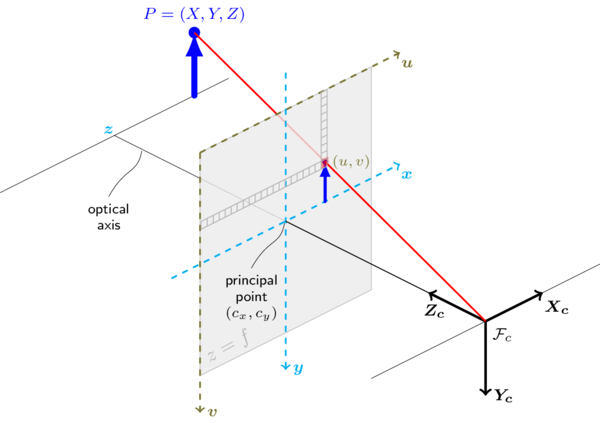
\includegraphics[width=.75\columnwidth]{pinhole.png}
\caption{Modelo de Câmera Estenopeica\cite{docsopencv}}
\end{center}
\end{figure}
reconstruction of both cameras and scene structure can be computed from image point correspondences alone; no other information is required. This answers both the second and third questions simultaneously. The reconstruction obtained from point correspondences alone is up to a projective ambiguity of 3-space, and this ambiguity can be resolved by supplying well defined additional information on the cameras or scene. In this manner an affine or metric reconstruction may be computed from uncalibrated images. T
Se os pontos do mundo \(X\) e da imagem \(x\) são representados por coordenadas homogêneas, podemos expressar matematicamente a projeção da câmera como uma matriz\cite{tese}:

\begin{equation}\lambda  x = P  X\label{eq:P_X}\end{equation}

onde \(\lambda\) é um fator de escala e P é a matriz 3x4 de projeção, também chamada matriz de calibração.

P pode ser decomposta em duas entidades geométricas: os parâmetros intrísecos \(K\) e extrínsecos \(R\) e \(t\) de calibração\cite{tese}
\begin{equation}
P = K [R | t]
\end{equation}
\begin{equation}
t = -R\widetilde{C}
\end{equation}
onde \(\widetilde{C}\) é a origem do sistema de coordenadas da câmera\cite{Hartley2004}.

Os parâmetros intrísecos de calibração descrevem a transformação entre a imagem ideal e a imagem em pixels
\begin{equation}
K = \begin{pmatrix} 
f & s & c_x \\
0 & \alpha f & c_y\\
0 & 0 & 1
\end{pmatrix}
\end{equation}
e os extrínsecos são a rotação \(R\) e translação \(t\) que transformam pontos no espaço do objeto para pontos no espaço da imagem\cite{tese}.

Como há 6 graus de liberdade nos parâmetros extrínsecos e 5 nos intrísecos, é necessário pelo menos 6 correspondências \({x_i \leftrightarrow X_i}\) do mesmo ponto no espaço da imagem e no espaço do objeto para obter P\cite{tese}. Mas dado que há um erro inerente nas medidas experimentais, para melhorar a qualidade da estimativa é preciso usar \(n > 6\) correspondências (como será visto em \ref{metodologia}, usaremos 48 pontos) e, assim, não há uma única matriz P que satisfaz esse sistema de equações. Precisamos, portanto, adicionar restrições para encontrar uma solução única.  

Um método comum é adicionar a restrição \(p_{34} = 0\)\cite{Hartley2004}, mas uma melhor abordagem\cite{tese} é:

\begin{equation}
\begin{aligned}
P = \min_{P'} \sum_{i}d(x_i, P'Xi)^2
\end{aligned}
\end{equation}
onde \(d(x_i, P'Xi) \) é a distância euclidiana entre o ponto observado e o estimado. 

\subsection{Projeção Reversa}
Ao projetar informações do mundo 3D para o 2D, \(P\) elimina informações do mundo real. Matematicamente podemos dizer que é uma matriz transformação 3x4, logo, não invertível. 

Dado um ponto na imagem, só é possível saber em que reta, a partir do centro da câmera, aquele ponto faz parte. Se, entretanto, estamos medindo um objeto que se encontra no mesmo plano em que foi feita a calibração, sabemos que \(Z=0\), e podemos calcular \(X\) a partir da \textit{Equação \ref{eq:P_X}} da seguinte forma:
\begin{equation}
\lambda  \begin{bmatrix} 
x \\
y \\
1
\end{bmatrix}
=
\begin{vmatrix} 
p_{11} & p_{12} & p_{13}=0& p_{14} \\
p_{21} & p_{22} & p_{23}=0& p_{24} \\
p_{31} & p_{32} & p_{33}=0& p_{34} 
\end{vmatrix}
\begin{bmatrix} 
X \\
Y \\
Z=0 \\
1
\end{bmatrix}
\end{equation}
\begin{equation}
\therefore  P_{3x3}^{-1} \lambda x = X
\end{equation}
\subsection{Distorções}

O modelo até aqui descrito descreve uma câmera ideal, mas as lentes das câmeras reais podem gerar distorções, que também são parâmetros intrínsecos que precisam ser considerados. 

A distorção radial é a mais importante e causa uma curvatura no mapeamento.

\begin{figure}[ht!]
\begin{center}
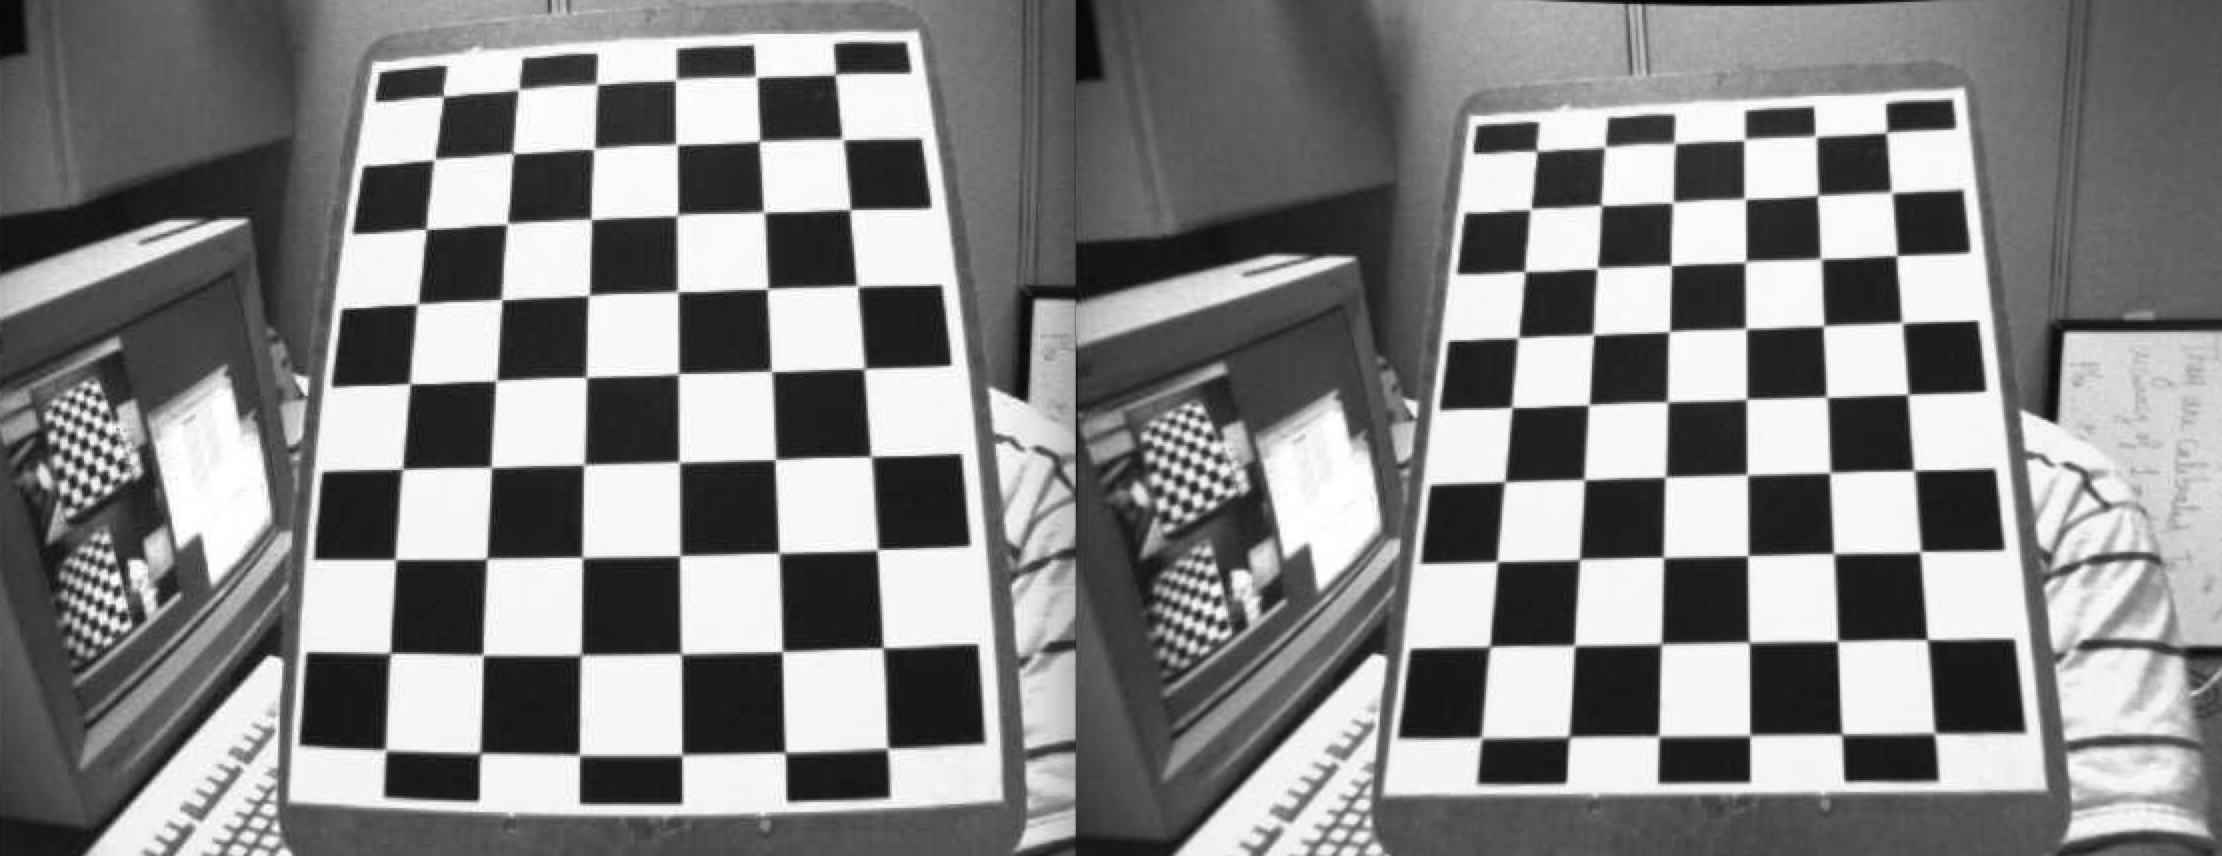
\includegraphics[width=\columnwidth]{distortion.png}
\caption{Distorção Radial\cite{docsopencv}}
\end{center}
\end{figure}

A correção dessa distorção pode ser modelada da seguinte maneira\cite{docsopencv}: 

    \[x_{retificado} = x( 1 + k_1 r^2 + k_2 r^4 + k_3 r^6)\]
    \[y_{retificado} = y( 1 + k_1 r^2 + k_2 r^4 + k_3 r^6)\]

Outra distorção comum é a tangencial, que ocorre quando o plano da lente não está alinhado. Para corrigir:


\[x_{retificado} = x + [ 2p_1xy + p_2(r^2+2x^2)] \]
\[y_{retificado} = y + [ p_1(r^2+ 2y^2)+ 2p_2xy] \]


Esses cinco parâmetros são conhecidos como coeficientes de distorção
\((k_1 \hspace{10pt} k_2 \hspace{10pt} p_1 \hspace{10pt} p_2 \hspace{10pt} k_3)\)\cite{docsopencv}.

\section{Metodologia}\label{metodologia}
O modelo da câmera e seus parâmetros foram descritos na seção de Revisão Teórica. Nesta seção, descreve-se como estimá-los experimentalmente.

\subsection{Materiais}
Foram utilizados:
\begin{itemize}
\item uma tábua de compensado
\item papel contact
\item fita adesiva
\item um padrão de calibração xadrez impresso em papel A4
\item uma trena
\item uma régua
\item computador MacBook Pro (Retina, 13-inch, Early 2015), Processador Intel Core i5 2,7 GHz, 8GB de RAM
\item Python 3.6.3 :: Anaconda custom (64-bit)
\item OpenCV 3.4.0
\item sete programas em python especialmente desenvolvidos para o projeto. Todos estão disponíveis no repositório: \url{git@github.com:fredguth/unb-cv-3183.git}\label{repo}
\end{itemize}

\subsection{Preparação}
 \begin{enumerate}
 \item Imprime-se o padrão de calibração em folha A4 e o cola à tábua de compensado usando o Papel Contact.
 \item Com o programa \textit{requisito1.py}, abre-se uma imagem jpg e com cliques do mouse desenha-se um segmento de reta sobre a imagem entre o primeiro e o segundo clique, registrando-se a distância \(||p2 - p1||_2 \) na própria imagem aberta. 
 \end{enumerate}
\subsection{Obtenção dos parâmetros intrínsecos}
 \begin{enumerate}
  \item Executa-se o programa \textit{requisito2.capture.py} que abre um stream de vídeo e grava a imagem sempre que detecta os cantos dos quadrados no padrão de calibração de tabuleiro de xadrez. O programa pede o número do experimento e grava as imagens capturadas no diretório do mesmo.  Foram feitos 8 experimentos que geraram entre 25 e 70 imagens cada.
  \item Executa-se o programa \textit{requisito2.calibrate.py} para cada experimento. O programa detecta os cantos dos quadrados do padrão de calibração xadrez e refina essa detecção para obter os parâmetros intrínsecos K e os coeficientes de distorção. É importante mover o quadrado no campo de captura da câmera em diversas orientações e posições, em diferentes distâncias. Os parâmetros intrínsecos e coeficientes de distorção são automaticamente armazenados em arquivos xml nos diretórios dos respectivos experimentos.
\item Dado que já temos os coeficientes de distorção, com o programa \textit{requisito2.measure.py} retificamos as imagens da câmera e permitimos medir distâncias na imagem retificada em pixels. 
\item Após todos os experimentos executados, executa-se o programa \textit{requisito2.analyse.py} que gera a média e o desvio parão dos parâmetros intrísecos, salvando-os no diretório \textit{exp-0}.
\end{enumerate}
\subsection{Obtenção dos parâmetros extrínsecos}\label{extrinsecos}
\begin{enumerate}
\item Com a régua, mede-se o tamanho de um quadrado no padrão de calibração.
\item Executa-se o programa \textit{requisito3.py}, que computa a correspondencia entre pontos da imagem e do espaço do objeto, atribuindo como origem do sistema de coordenadas do mundo, o ponto de intersecção do canto superior esquerdo do tabuleiro e através da função \textit{solvePnP} da OpenCV\cite{OpenCV}, obtem os parâmetros extrínsecos R e t. 
\item Quando o programa pede o número do experimento, escolhe-se \(0\), uma vez que queremos usar os parâmetros intrísecos médios, medidos na etapa anterior.

\item Deixa-se a câmera em um ponto marcado pela fita adesiva, tentando colocá-la ortogonal ao plano da sua base. 
\item Com a câmera posicionada, posiciona-se o tabuleiro na distância mais próxima possível da câmera em que o padrão de calibração tem seus cantos detectados (os cantos ficam marcados com pontos coloridos no \textit{stream} da câmera), marcando com a fita adesiva este ponto como \(d_{min}\). \label{montagem}
\item Repete-se o passo anterior, tentando encontrar a distância mais afastada da câmera. Marca-se este ponto com fita adesiva como \(d_{max}\); e também um ponto intermediário entre \(d_{min}\) e \(d_{max}\), que chamamos \(d_{med}\).
\item Medimos as distâncias \(d_{min}\), \(d_{med}\)  e \(d_{max}\) com a trena.
\item Com todos os pontos marcados e a câmera posicionada, acionamos o modo de captura apertando a tecla \textit{espaço}
\item Leva-se o tabuleiro de xadrez para \(d_{min}\) e após algumas capturas (identificação do padrão xadrez na imagem \textit{stream} da câmera), apertamos a tecla \textit{espaço} novamente para sair do modo captura.\label{medicao}
\item Repete-se os últimos dois passos para as distâncias \(d_{med}\) e \(d_{med}\). As imagens captadas com as respectivas distâncias medidas são gravadas no diretório do experimento selecionado. É importante verificar se há pelo menos 3 imagens gravadas para cada distância.
\end{enumerate}
\subsection{Obtenção da altura de um objeto através da sua imagem}
\begin{enumerate}
\item Executa-se o programa \textit{requisito4.py} e posiciona-se o padrão de calibração no plano onde se deseja colocar o objeto (é recomendável marcar esse ponto com a fita inicialmente).
\item Com a câmera calibrada, posiciona-se o objecto que se deseja medir no plano de calibração marcado pela fita.
\item Com o mouse, clica-se na imagem dos extremos do objeto, formando linhas entre os extremos (cima a baixo e esquerda e direita).
\item Com a régua, confere-se as medidas reais entre os extremos.
\end{enumerate}
Com os parâmetros intrínsecos e extrínsecos,  é possível medir um objeto no mundo real a partir da sua imagem. Neste projeto, entretanto, não se obteve êxito em desenvolver essa funcionalidade no programa \textit{requisito4.py}

\section{Resultados}
Nesta seção apresentamos, para cada etapa da \ref{metodologia}, os resultados obtidos. Todos os dados podem ser acessados no repositório do projeto (\ref{repo}).
\subsection{Medição em pixels de segmentos de imagens}
\begin{figure}[ht!]\label{baboon}
\begin{center}
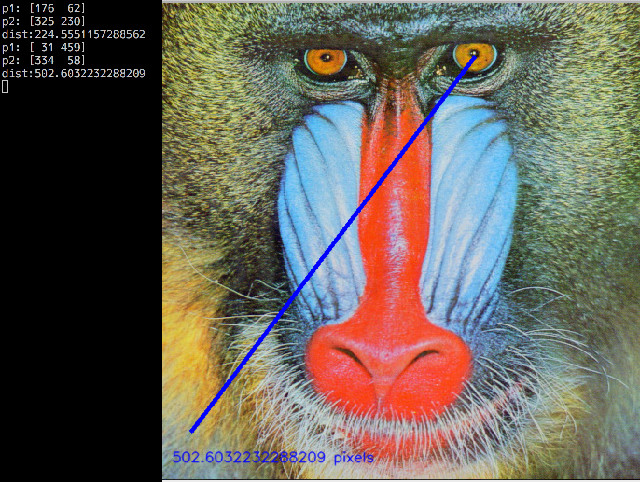
\includegraphics[width= .5\columnwidth]{baboon.jpg}
\caption{Medição em pixels de segmentos em imagens}
\end{center}
\end{figure}
A figura \ref{baboon} mostra a medição em pixels de segmentos entre cliques na imagem. Além da saída no \textit{console}, o programa mostra a distância em pixels na própria tela.
\subsection{Calibração dos parâmetros intrínsecos}

A figura \ref{snapshots} mostra diversas das imagens captadas para calibração, onde tentou-se explorar ao máximo a diferença de posição, distância e até luminosidade do ambiente.
\begin{figure}[!htb]\label{snapshots}
\minipage{0.33\columnwidth}
  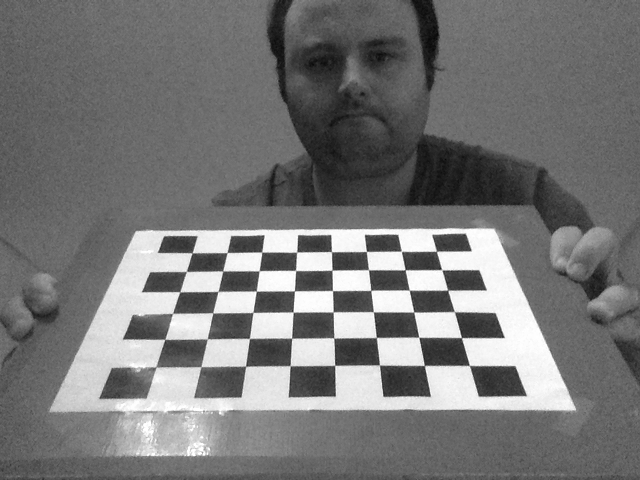
\includegraphics[width=\linewidth]{snap-1.png}
\endminipage\hfill
\minipage{0.33\columnwidth}
  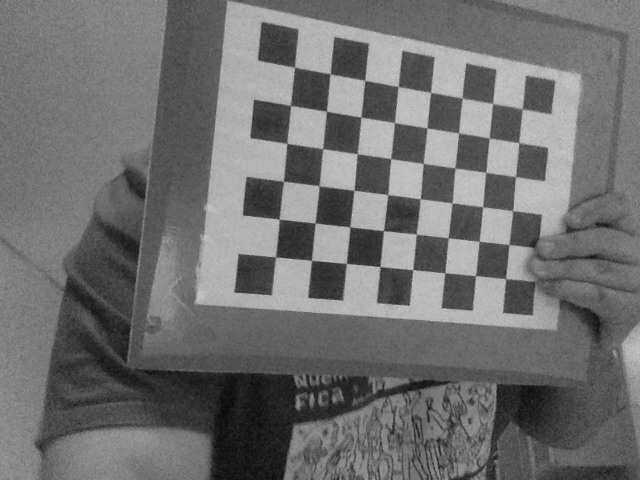
\includegraphics[width=\linewidth]{snap-2.png}
\endminipage\hfill
\minipage{0.33\columnwidth}%
  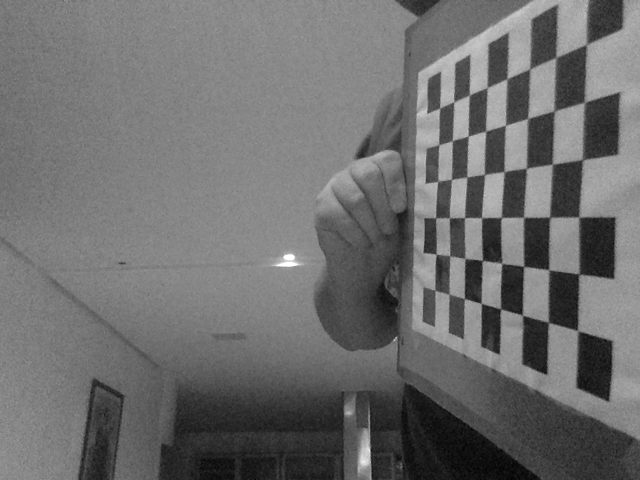
\includegraphics[width=\linewidth]{snap-3.png}
\endminipage\hfill
\minipage{0.33\columnwidth}
  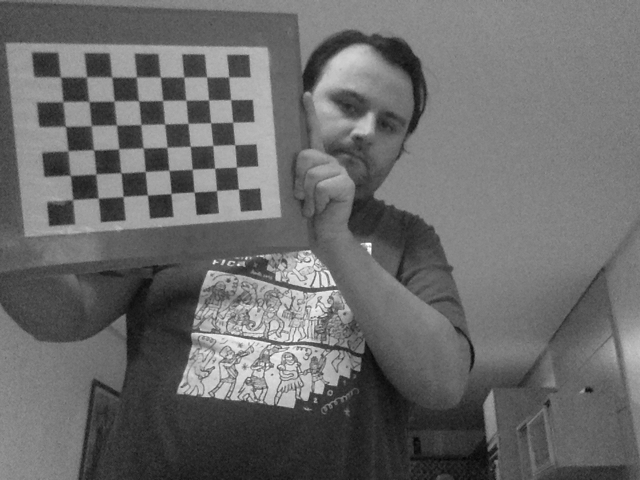
\includegraphics[width=\linewidth]{snap-4.png}
\endminipage\hfill
\minipage{0.33\columnwidth}
  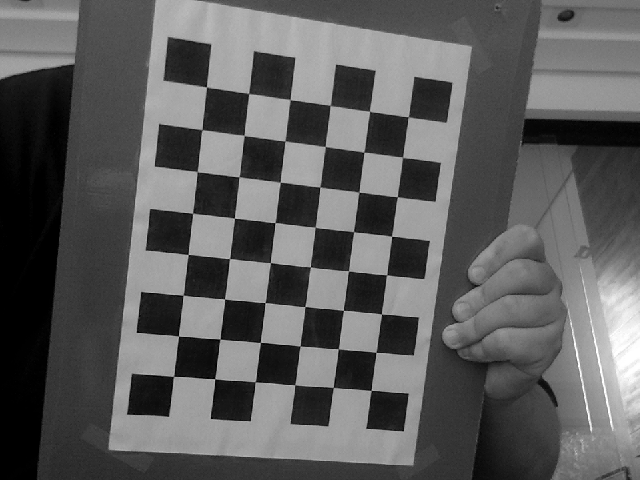
\includegraphics[width=\linewidth]{snap-5.png}
\endminipage\hfill
\minipage{0.33\columnwidth}%
  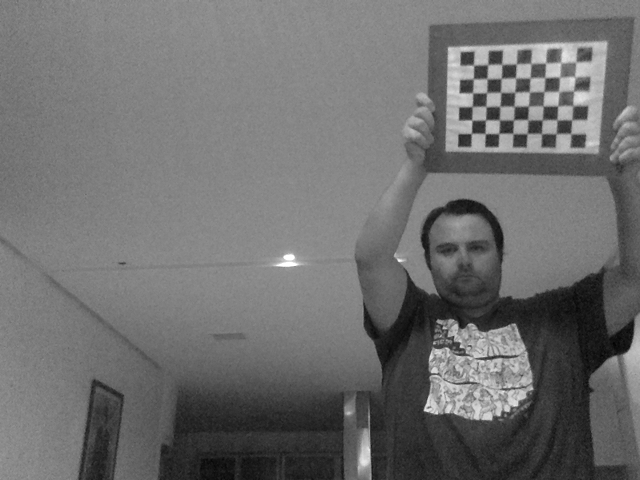
\includegraphics[width=\linewidth]{snap-6.png}
\endminipage\hfill
\caption{Algumas das dezenas de \textit{snapshots} geradas em diferentes posições}
\end{figure}
O resultado obtido para os parâmetros intrínsecos foram:
$$
K = \begin{pmatrix} 
673.08 & 0 & 312.32 \\
0 & 668.10 & 236.50\\
0 & 0 & 1
\end{pmatrix}
\pm
\begin{pmatrix} 
56.27 & 0 & 13.24 \\
0 & 55.75 & 22.71\\
0 & 0 & 1
\end{pmatrix}
$$
\((k_1=0.150\pm0.039 \hspace{10pt} k_2=-.744\pm0.448 \hspace{10pt} p_1=0.003\pm0.003 \hspace{10pt} p_2=-0.003\pm0.007 \hspace{10pt} k_3=1.820\pm1.932)\)
\subsection{Calibração dos parâmetros extrínsecos}\label{calibextr}
Na figura \ref{extr} mostramos como foram capturadas as imagens para obtenção dos parâmetros extrínsecos.
\begin{figure}\label{extr}
\centering
\begin{minipage}{.45\columnwidth}
  \centering
  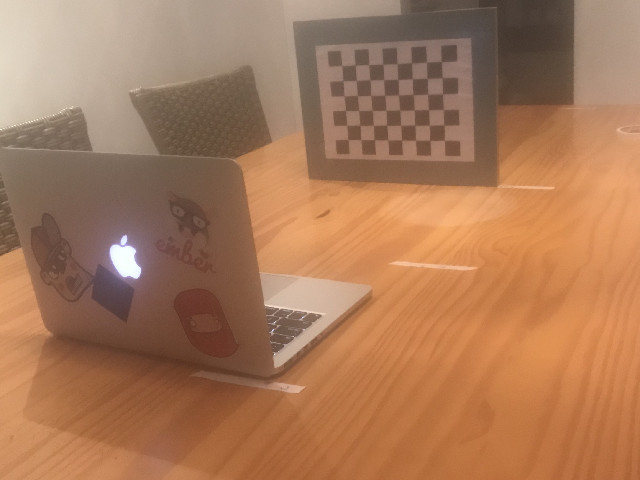
\includegraphics[width=.95\linewidth]{cena.jpg}
  \caption{Montagem \ref{extrinsecos}.\ref{montagem}}
  \label{fig:test1}
\end{minipage}%
\begin{minipage}{.45\columnwidth}
  \centering
  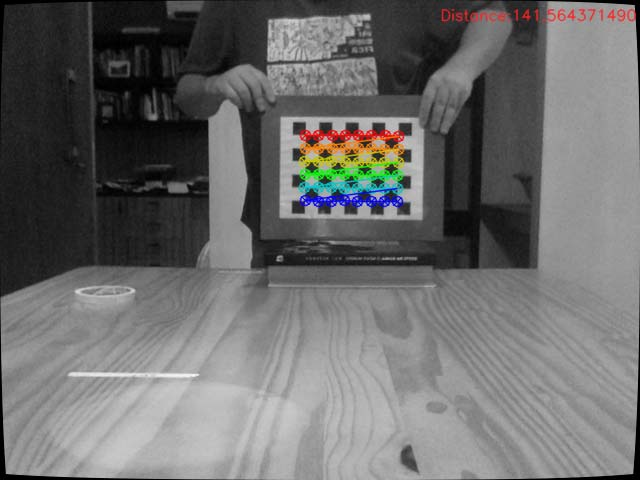
\includegraphics[width=.95\linewidth]{extr.jpg}
  \caption{Medição \ref{extrinsecos}.\ref{medicao}}
  \label{fig:test2}
\end{minipage}
\end{figure}
O resultado está apresentado na tabela \ref{distancias}.
\begin{table}[htbp]\label{distancias}
\caption{Comparação distâncias estimadas versus real}
\begin{center}
\begin{tabular}{|c|c|c|c|c|c|c|}
\hline
em \textit{cm}& \textbf{\textit{Real}}& \(d_{1}\)&\(d_{1}\)&\(d_{3}\)&\(\bar{d}\)& \textbf{\(\sigma\)} \\
\hline
\(d_{min}\)& 32.3& 31.35& 31.93 & 31.97& 31.75& 0.35\\
\hline
\(d_{med}\)& 72.3& 69.51& 68.87 & 68.57& 68.98& 0.48\\
\hline
\(d_{max}\)& 148.1& 138.78& 141.87 & 144.31& 141.65& 2.77\\
\hline

\end{tabular}
\label{tab1}
\end{center}
\end{table}
O erro ficou entre 2 e 6\%. Um pouco acima da margem de 2\% do desvio padrão.
\subsection{Medição de Objeto 3D a partir de sua imagem}
\begin{figure}[ht!]\label{baboon}
\begin{center}
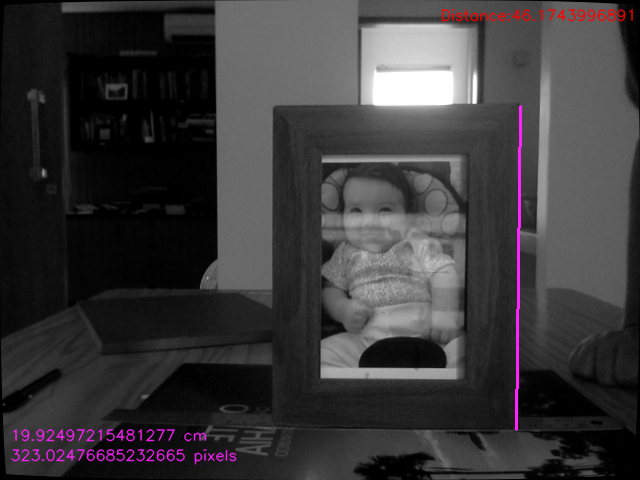
\includegraphics[width= .9\columnwidth]{projection-2.png}
\caption{Medição em pixels de segmentos em imagens}
\end{center}
\end{figure}
\section{Discussão e Conclusões}
Neste trabalho, utilizamos o modelo de câmera estenopeica para fazer mapeamentos de posições no mundo real para a imagem e vise-versa. O resultado obtido para as distâncias \ref{calibextr} na calibração dos parâmetros extrínsecos tiveram um erro menor do que 6\%. Entretanto, cabe ressaltar que para isso foi necessário capturar centenas de imagens na fase de calibração dos intrínsecos. Tentativas feitas que usavam poucas dezenas não lograram êxito. 

% \begin{figure}[htbp]
% \centerline{
\includegraphics{fig.jpg}}
% \caption{Example of a figure caption.}
% \label{fig}
% \end{figure}

\selectlanguage{brazilian}
\bibliographystyle{IEEEtran}
\bibliography{references}

\end{document}
